\section{Introduction}\label{sec:introduction}
%%%%%%%%%%%%%%%%%%%%%%%%%%%%%%%%%%%%%%%%
%%%%%%%%Introduction and Problems%%%%%%%%
%%%%%%%%%%%%%%%%%%%%%%%%%%%%%%%%%%%%%%%%

Vector quantization (VQ)~\cite{Oord2017NeuralDR} is a fundamental building block in a wide range of modern representation learning and visual tokenization frameworks, including autoregressive and hybrid generative models~\cite{Razavi2019GeneratingDH,Esser2020TamingTF,Chang2022MaskGITMG,Lee2022AutoregressiveIG,Gu2021VectorQD,Tian2024VisualAM,Li2024XQGANAO}. By discretizing continuous feature representations using a learnable codebook, VQ enables compact and structured latent representations that are well suited for downstream modeling. Despite its broad adoption, VQ remains notoriously difficult to optimize in practice, often exhibiting unstable training dynamics and severe codebook collapse.


The first challenge stems from the non-differentiability of the quantization operation, which prevents gradients from being directly propagated from quantized features to their continuous counterparts. To address this issue, prior work introduces the straight-through estimator (STE)~\cite{bengio2013estimating,Oord2017NeuralDR}, which approximates gradients by copying them from the quantized features to encoder outputs. However, the effectiveness of this approximation critically depends on the magnitude of the quantization error. When the discrepancy between continuous features and their assigned code vectors becomes large, the resulting gradient mismatch can lead to unstable optimization and degraded training behavior~\cite{Lee2022AutoregressiveIG}.



A second, closely related challenge is codebook collapse, where only a small subset of code vectors receives assignments while the majority remain unused. From a geometric perspective, this corresponds to a degenerate Voronoi partition\footnote{Appendix.~\ref{appendix:understanding codebook collapse by Voronoi Partition} discusses codebook collapse via Voronoi partitioning.} in which most cells are never activated~\cite{Zheng2023OnlineCC}. Although extensive research has sought to alleviate this problem, low code vector utilization often remains in practice, particularly with large codebooks~\cite{Dhariwal2020JukeboxAG,Takida2022SQVAEVB,Yu2021VectorquantizedIM,Lee2022AutoregressiveIG,Zheng2023OnlineCC}. This limitation is further exacerbated as increasing the codebook size expands the number of Voronoi cells, making it substantially harder to ensure that all cells are sufficiently populated.




\begin{wrapfigure}[12]{r}{0.54\textwidth}
\small
\vspace{-6mm}
\begin{center}
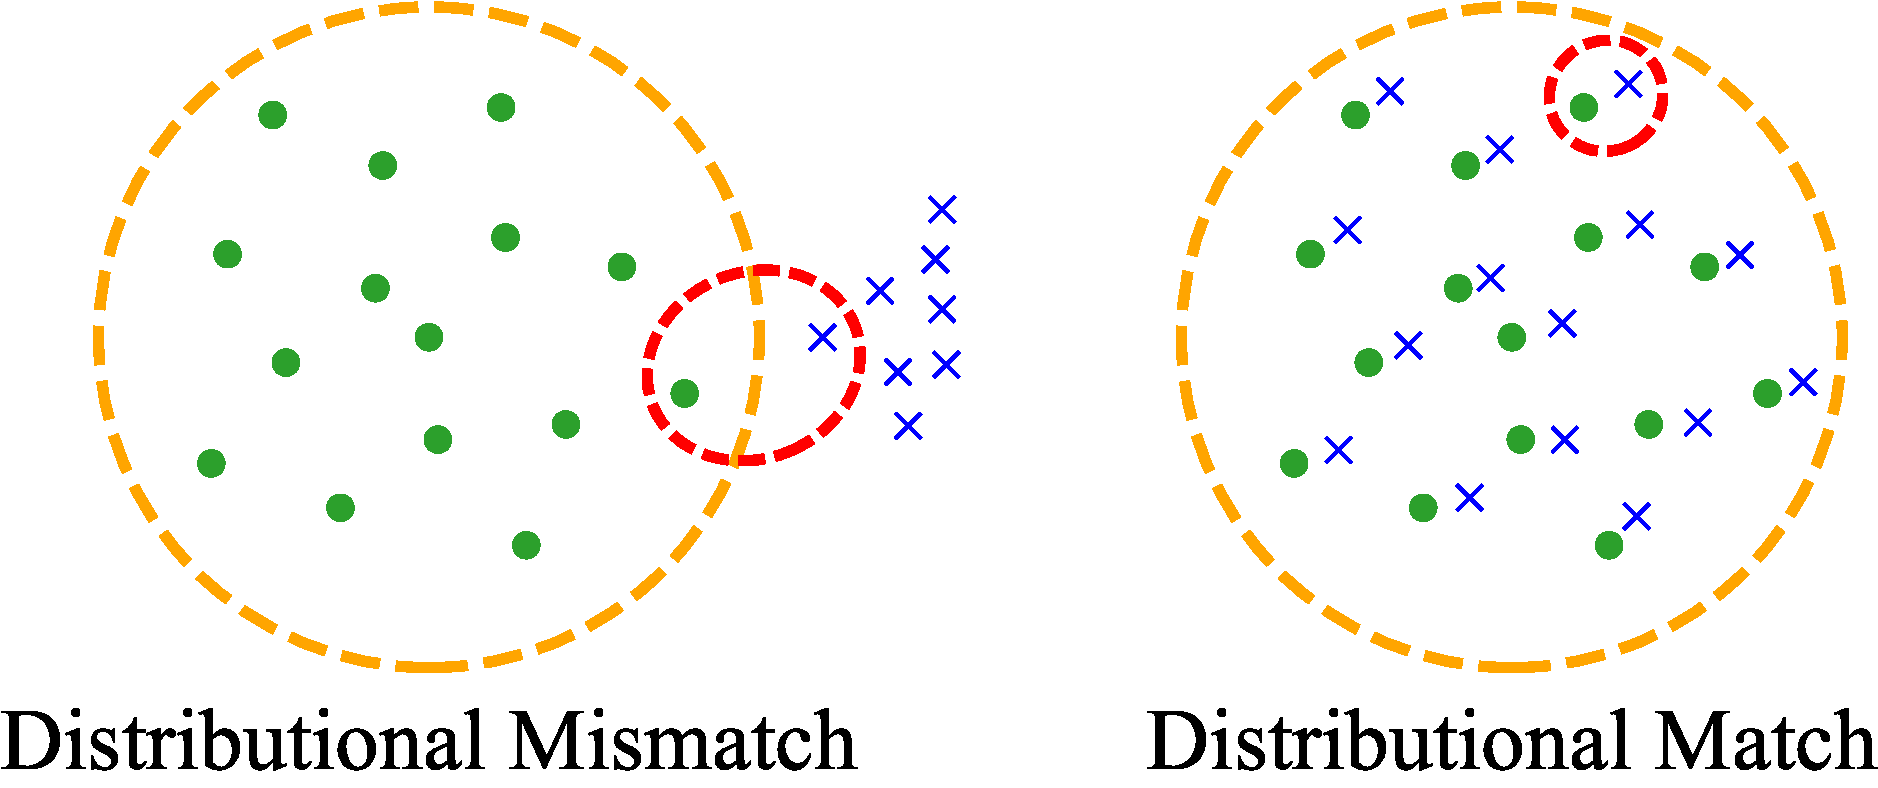
\includegraphics[width=0.52\textwidth]{figs/architecture/distribution_comparison.pdf}
\vspace{-2mm}
\caption{\small{The symbols $\cdot$ and $\times$ represent the feature and code vectors, respectively. The left figure illustrates the distributional mismatch between the feature and code vectors, while the right figure visualizes their distributional match.}}
\label{fig:distributional match}
\end{center}
\end{wrapfigure} 
In this work, we examine these challenges from a distributional perspective. Rather than treating training instability and codebook collapse as separate phenomena, we observe that both issues are closely tied to a fundamental mismatch between the distributions of feature vectors produced by the encoder and the distributions of the learnable code vectors. Figure~\ref{fig:distributional match} illustrates this intuition using two representative scenarios. When the two distributions are poorly aligned, feature vectors concentrate around a small subset of code vectors, resulting in large quantization errors and low codebook utilization. In contrast, when the distributions are well matched, quantization errors are reduced and codebook utilization approaches its maximum.




Building on this observation, we introduce three principled criteria that characterize the desirable behavior in vector quantization. Guided by this criterion triple, we show through both theoretical analysis and empirical evaluation that distributional alignment between feature vectors and code vectors provides a unifying mechanism for mitigating training instability and codebook collapse. To operationalize this idea, we adopt a distribution matching objective based on the quadratic Wasserstein distance. Under a mild Gaussian approximation, this objective admits a closed-form expression that can be efficiently optimized during training. Importantly, we show that even when this approximation is relaxed, a nonparametric alternative based on maximum mean discrepancy (MMD)~\cite{Gretton2012AKT, Sriperumbudur2009HilbertSE,Fang2025VQTransplant} yields comparable performance, suggesting that distributional matching effectively captures the essential structure required for effective vector quantization. These insights translate into consistent improvements in reconstruction fidelity across visual tokenization benchmarks.





% \textcolor{red}{Our contributions are summarized as follows:
% \begin{itemize}
%     \item We identify distributional mismatch between feature vectors and code vectors as a unifying cause of training instability and codebook collapse in vector quantization.
%     \item We introduce a principled criterion triple that characterizes desirable behavior in VQ and use it to analyze existing methods.
%     \item We show theoretically and empirically that distributional alignment provides an effective mechanism for improving optimization stability and codebook utilization.
%     \item We propose an efficient distribution matching objective based on the quadratic Wasserstein distance, along with a nonparametric MMD variant that relaxes distributional assumptions.
%     \item We demonstrate strong empirical results on visual tokenization benchmarks, achieving near-complete codebook utilization and improved reconstruction quality with minimal overhead.
% \end{itemize}
% }

%%%%Our contributions%%%%%%
%%% this is a bit repeatative of the above content?
%Our main contributions are summarized as follows: (i) We introduce a new distributional perspective on VQ, providing a framework to optimize VQ processes. (ii) We identify three principled criteria that collectively form a criterion {triple}, which characterizes an optimal VQ solution. (iii) We present robust empirical and theoretical evidence demonstrating that distribution matching closely approximates the optimal solution for VQ. (iv) We propose using Wasserstein distance to achieve the distributional match, effectively addressing both training instability and codebook collapse issues.


%Our main contributions are summarized as follows: (1) We propose a new distributional perspective to examine the training instability and codebook collapse issues in existing VQ methods. (2) We introduce three principled criteria as evaluation metrics for assessing VQ methods. (3) Our comprehensive empirical studies suggest that these critiria are optimized when the distributions of feature vectors and code vectors are identical. (4) We provide theoretical analysis supporting  distributional alignment.  (5) We propose to use the quadratic  Wasserstein distance to achieve this alignment, effectively addressing both training instability and codebook collapse issues.


%and theoretical evidence suggesting that distribution matching closely approximates the optimal solution for VQ. (4) We propose using Wasserstein distance to achieve the distributional match, effectively addressing both training instability and codebook collapse issues.


